
%(BEGIN_QUESTION)
% Copyright 2006, Tony R. Kuphaldt, released under the Creative Commons Attribution License (v 1.0)
% This means you may do almost anything with this work of mine, so long as you give me proper credit

An orifice plate is used to measure the flow rate of ultra-pure water at a pharmaceuticals processing facility where the customary unit for liquid flow measurement is ``liters per minute'' (LPM).  Calculate the following parameters in this flow measurement loop, at two different flow rates (78 LPM and 120 LPM):

$$\includegraphics[width=15.5cm]{i00726x01.eps}$$

Note that the transmitter is equipped with internal square root characterization, so that no external square root computer is required.

\begin{itemize}
\item {} {\bf At a flow rate of 78 LPM:}
\vskip 5pt
\item{} Orifice plate $\Delta$P = \underbar{\hskip 50pt} " H$_{2}$O
\vskip 5pt
\item{} Differential pressure transmitter output signal = \underbar{\hskip 50pt} mA
\vskip 5pt
\item{} Flow indicator reading = \underbar{\hskip 50pt} LPM
\end{itemize}

\vskip 10pt

\begin{itemize}
\item {} {\bf At a flow rate of 120 LPM:}
\vskip 5pt
\item{} Orifice plate $\Delta$P = \underbar{\hskip 50pt} " H$_{2}$O
\vskip 5pt
\item{} Differential pressure transmitter output signal = \underbar{\hskip 50pt} mA
\vskip 5pt
\item{} Flow indicator reading = \underbar{\hskip 50pt} LPM
\end{itemize}

\vskip 20pt \vbox{\hrule \hbox{\strut \vrule{} {\bf Suggestions for Socratic discussion} \vrule} \hrule}

\begin{itemize}
\item{} A poor choice of flowmeters for this particular application would be {\it magnetic}.  Explain why
\end{itemize}

\underbar{file i00726}
%(END_QUESTION)





%(BEGIN_ANSWER)

$$Q = k \sqrt{\Delta P}$$

At a volumetric flow rate of 200 liters per minute and a corresponding differential pressure of 100 "WC, the value of $k$ will be 20.

\begin{itemize}
\item {} {\bf At a flow rate of 78 LPM:}
\vskip 5pt
\item{} Orifice plate $\Delta$P = \underbar{\bf 15.21} " H$_{2}$O
\vskip 5pt
\item{} Differential pressure transmitter output signal = \underbar{\bf 10.24} mA
\vskip 5pt
\item{} Flow indicator reading = \underbar{\bf 78} LPM
\end{itemize}

\vskip 10pt

\begin{itemize}
\item {} {\bf At a flow rate of 120 LPM:}
\vskip 5pt
\item{} Orifice plate $\Delta$P = \underbar{\bf 36} " H$_{2}$O
\vskip 5pt
\item{} Differential pressure transmitter output signal = \underbar{\bf 13.6} mA
\vskip 5pt
\item{} Flow indicator reading = \underbar{\bf 120} LPM
\end{itemize}


%(END_ANSWER)





%(BEGIN_NOTES)



%INDEX% Measurement, flow: orifice plate loop calculations

%(END_NOTES)


